% Copyright 2004 by Till Tantau <tantau@users.sourceforge.net>.
%
% In principle, this file can be redistributed and/or modified under
% the terms of the GNU Public License, version 2.
%
% However, this file is supposed to be a template to be modified
% for your own needs. For this reason, if you use this file as a
% template and not specifically distribute it as part of a another
% package/program, I grant the extra permission to freely copy and
% modify this file as you see fit and even to delete this copyright
% notice. 

\documentclass{beamer}

% There are many different themes available for Beamer. A comprehensive
% list with examples is given here:
% http://deic.uab.es/~iblanes/beamer_gallery/index_by_theme.html
% You can uncomment the themes below if you would like to use a different
% one:
%\usetheme{AnnArbor}
%\usetheme{Antibes}
%\usetheme{Bergen}
%\usetheme{Berkeley}
%\usetheme{Berlin}
%\usetheme{Boadilla}
%\usetheme{boxes}
%\usetheme{CambridgeUS}
%\usetheme{Copenhagen}
%\usetheme{Darmstadt}
%\usetheme{default}
%\usetheme{Frankfurt}
%\usetheme{Goettingen}
%\usetheme{Hannover}
%\usetheme{Ilmenau}
%\usetheme{JuanLesPins}
%\usetheme{Luebeck}
\usetheme{Madrid}
\usepackage{graphicx}
\usepackage{textpos}
%\usetheme{Malmoe}
%\usetheme{Marburg}
%\usetheme{Montpellier}
%\usetheme{PaloAlto}
%\usetheme{Pittsburgh}
%\usetheme{Rochester}
%\usetheme{Singapore}
%\usetheme{Szeged}
%\usetheme{Warsaw}
\usepackage{CJKutf8}

\CJKencfamily{UTF8}{bkai}

\AtBeginDocument{%
    \begin{CJK}{UTF8}{bkai}} 
    \AtEndDocument{%
    \clearpage\end{CJK}}

\title{iWildCam 2019 - FGVC6}

% A subtitle is optional and this may be deleted
\subtitle{Categorize animals in the wild}

\author{F.~黃騰陞\inst{1} \and S.~吳宗晉\inst{2} \and T.~施紹唐\inst{3}}
% - Give the names in the same order as the appear in the paper.
% - Use the \inst{?} command only if the authors have different
%   affiliation.

\institute[Universities of Somewhere and Elsewhere] % (optional, but mostly needed)
{
  \inst{1}%
  Department of Computer Science\\
  University of Yuan Ze
}
% - Use the \inst command only if there are several affiliations.
% - Keep it simple, no one is interested in your street address.

\date{開放平台軟體期末專題, 2019}
% - Either use conference name or its abbreviation.
% - Not really informative to the audience, more for people (including
%   yourself) who are reading the slides online

\subject{Theoretical Computer Science}
% This is only inserted into the PDF information catalog. Can be left
% out. 

% If you have a file called "university-logo-filename.xxx", where xxx
% is a graphic format that can be processed by latex or pdflatex,
% resp., then you can add a logo as follows:

% \pgfdeclareimage[height=0.5cm]{university-logo}{university-logo-filename}
% \logo{\pgfuseimage{university-logo}}

% Delete this, if you do not want the table of contents to pop up at
% the beginning of each subsection:
\AtBeginSubsection[]
{
  \begin{frame}<beamer>{Outline}
    \tableofcontents[currentsection,currentsubsection]
  \end{frame}
}

% Let's get started
\begin{document}
\begin{CJK}{UTF8}{}
\begin{frame}
  \titlepage
\end{frame}

\begin{frame}{Outline}
\setcounter{tocdepth}{1}
  \tableofcontents
  % You might wish to add the option [pausesections]
\end{frame}

% Section and subsections will appear in the presentation overview
% and table of contents.
\section{Introduction}

\subsection{成員介紹}

\begin{frame}{Introduction}{成員介紹}
  \begin{itemize}
  \item {
    1043362 黃騰陞
  }
  \item {
    1041562 吳宗晉
  }
  \item {
    1043310 施紹唐	
  }
  \end{itemize}
\end{frame}

\subsection{專題問題描述}

% You can reveal the parts of a slide one at a time
% with the \pause command:
\begin{frame}{Introduction}{專題問題描述}
  \begin{itemize}
  \item {
    我們挑選的主題是Categorize animals in the wild,一個在kaggle上面舉辦的比賽,利用kaggle提供的資料集來訓練出一個模型,讓我們可以藉由這個模型來為輸入影像分類,模型可以區分22種動物,希望可以藉由訓練出模型來監測觀察不同地區生物生態以及遷移情況,讓研究人員可以更輕易的掌握生態變遷。

    %\pause % The slide will pause after showing the first item
  }
  
  \end{itemize}
\end{frame}

\section{Methodology}

\subsection{Input of model}

\begin{frame}{Methodology}{Input of model}.
\vspace{-4.5cm}
	\begin{itemize}
	\item{
		一個(32,32,3)圖片
		\begin{textblock}{3}(1,1)
		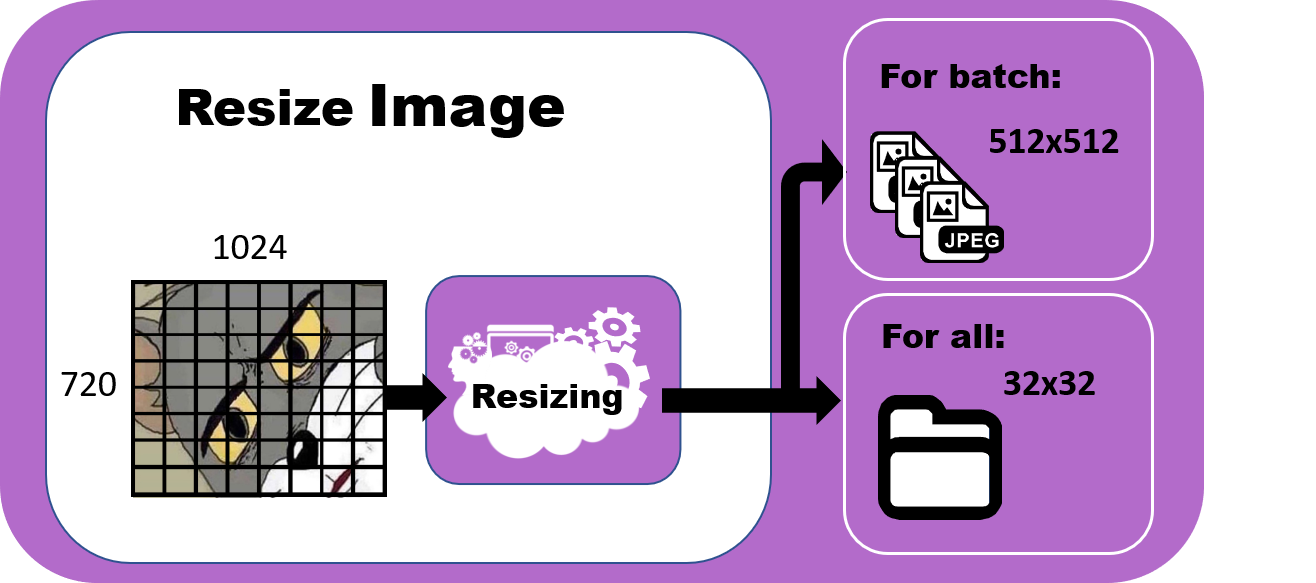
\includegraphics[width=5.5cm]{resize.png}
		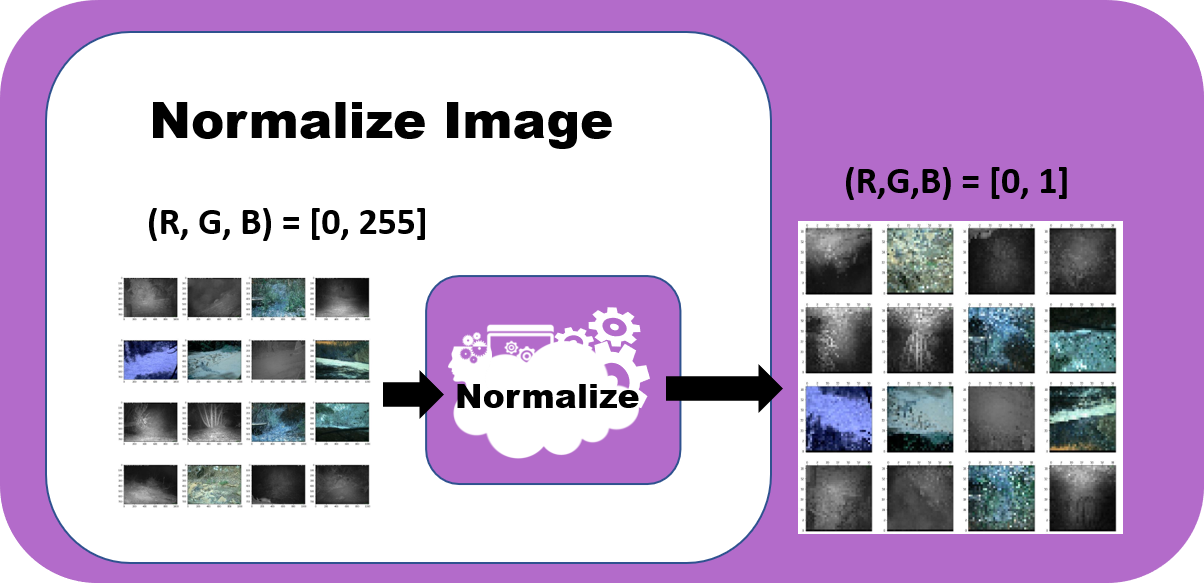
\includegraphics[width=5cm]{normalize.png}
		\end{textblock}
	}
	
	
	\end{itemize}
\end{frame}

\subsection{Output of model}

\begin{frame}{Methodology}{Output of model}
\vspace{-4.5cm}
	\begin{itemize}
	\item{
		輸出一個權重檔案,model.h5
		\begin{textblock}{3}(1,1)
		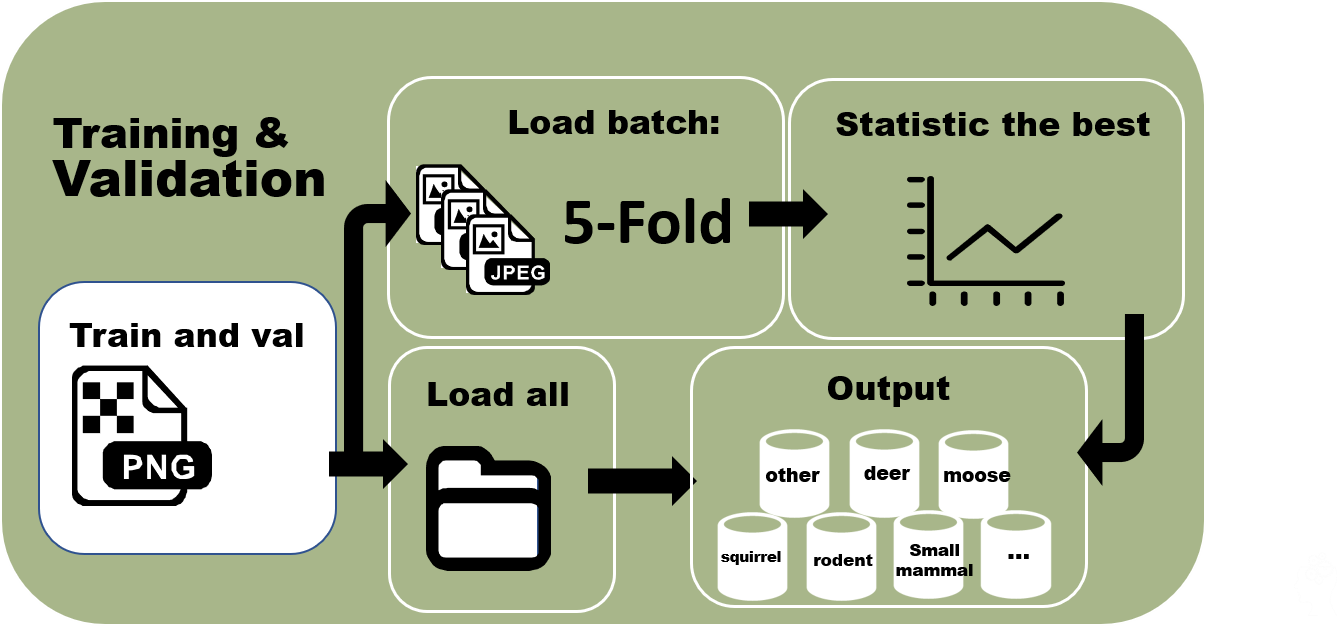
\includegraphics[width=10cm]{output.png}
		\end{textblock}
	}
	\end{itemize}
\end{frame}

\subsection{Layers of model}

\begin{frame}{Methodology}{Layers of model}
	\begin{itemize}
	\item{
		Dense121\\
		GlobalAveragePooling2D(池化層)\\
		激活函數(將輸出轉為機率)\\
	}
	\end{itemize}
\end{frame}

\subsection{Model save}

\begin{frame}{Methodology}{Model save}
	\begin{itemize}
	\item{
		使用ModelCheckpoint函式儲存框架以及權重
	}
	\end{itemize}
\end{frame}

\subsection{File size of model}

\begin{frame}{Methodology}{File size of model}
\vspace{-4.5cm}
	\begin{itemize}
	\item{
		\begin{textblock}{3}(1,1)
		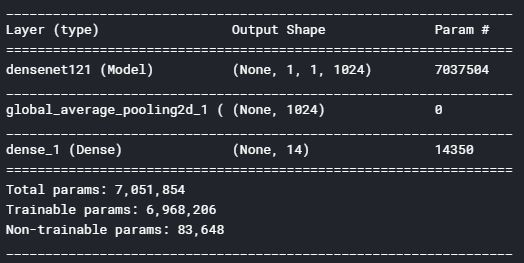
\includegraphics[width=10cm]{file_size_of_model.png}
		\end{textblock}
	}
	\end{itemize}
\end{frame}

\subsection{Loss function}

\begin{frame}{Methodology}{Loss function}
	\begin{itemize}
	\item{
		使用categorical crossentropy loss function\\
		因為我們在最後一層使用softmax激活函數計算機率,通常會搭配categorical crossentropy loss function 使用\\ 
	}
	\end{itemize}
\end{frame}

\subsection{Optimizer and hyperparameter}

\begin{frame}{Methodology}{Optimizer and hyperparameter}
	\begin{itemize}
	\item{
		Optimizer使用adam\\
		沒有使用hyperparameter
	}
	\end{itemize}
\end{frame}

\section{Dataset}

\subsection{Size of dataset}

\begin{frame}{Dataset}{資料集大小}
\vspace{-4.5cm}
	\begin{itemize}
	\item{
		kaggle 競賽提供的資料集43G
		\begin{textblock}{3}(1,1)
		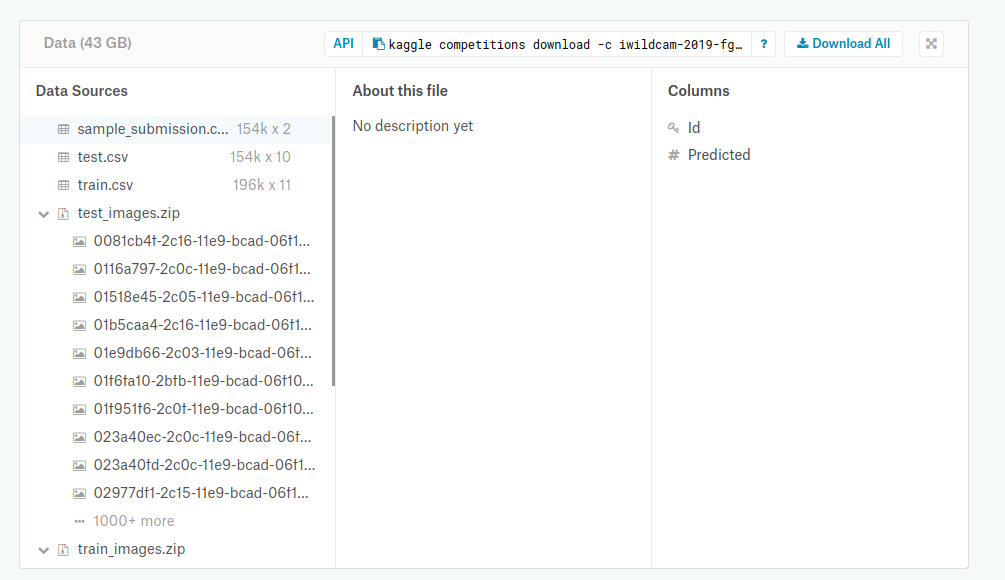
\includegraphics[width=10cm]{dataset.png}
		\end{textblock}
	}
	\end{itemize}
\end{frame}

\subsection{資料集來源}

\begin{frame}{Dataset}{資料集來源}
\vspace{-4.5cm}
	\begin{itemize}
	\item{
		kaggle 競賽提供
		\begin{textblock}{3}(1,1)
		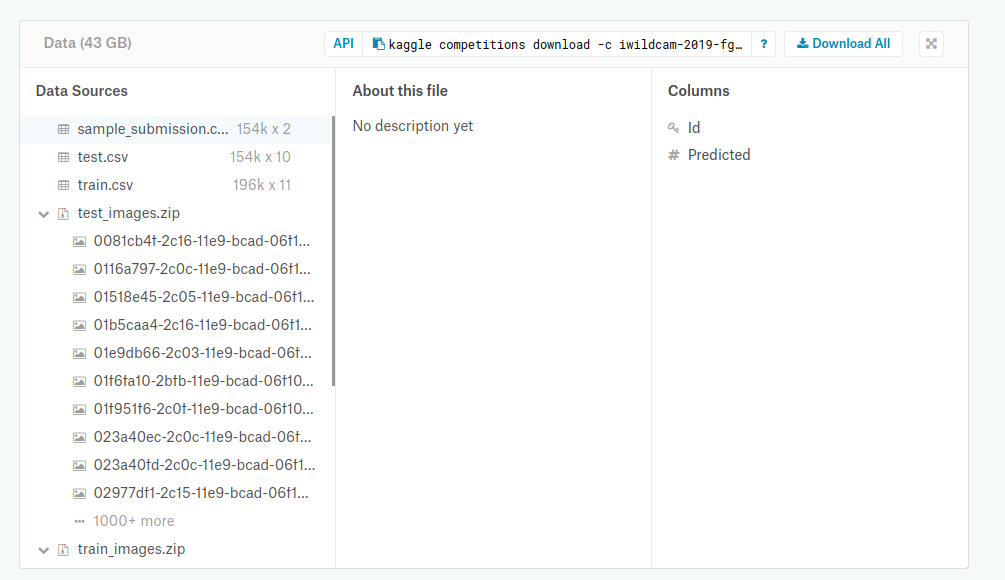
\includegraphics[width=10cm]{dataset.png}
		\end{textblock}
		%在一張圖片
	}
	\end{itemize}
\end{frame}

\subsection{訓練樣本數量}

\begin{frame}{Methodology}{訓練樣本數量}
\vspace{-4.5cm}
	\begin{itemize}
	\item{
		130862張圖片
		\begin{textblock}{3}(1,1)
		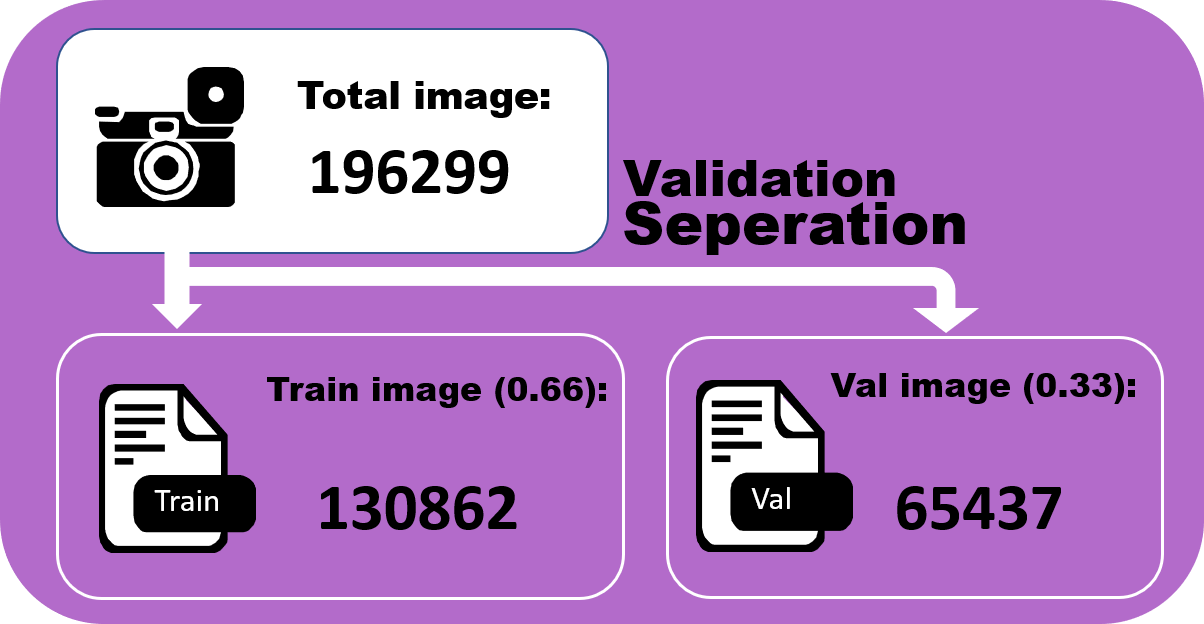
\includegraphics[width=10cm]{data_split.png}
		\end{textblock}
	}
	\end{itemize}
\end{frame}

\subsection{驗證樣本數量}

\begin{frame}{Dataset}{驗證樣本數量}
\vspace{-4.5cm}
	\begin{itemize}
	\item{
		65437張圖片
		\begin{textblock}{3}(1,1)
		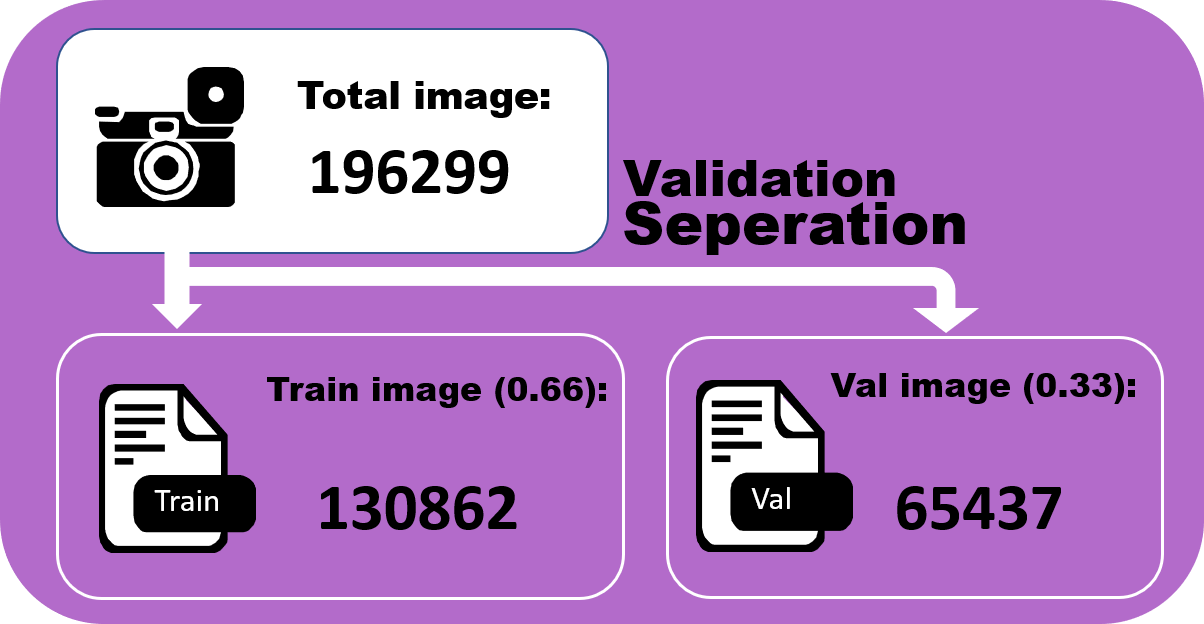
\includegraphics[width=10cm]{data_split.png}
		\end{textblock}
	}
	\end{itemize}
\end{frame}

\subsection{測試樣本數量}

\begin{frame}{Dataset}{測試樣本數量}
	\begin{itemize}
	\item{
		153730張圖片
	}
	\end{itemize}
\end{frame}

\section{Experimental Evaluation}

\subsection{Experimental environment}

\begin{frame}{Experimental Evaluation}{Experimental environment}
\vspace{-4.5cm}
	\begin{itemize}
	\item{
		kaggle 競賽提供的kernel
		\begin{textblock}{3}(1,1)
		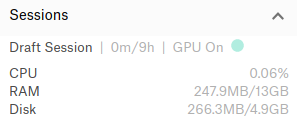
\includegraphics[width=10cm]{kernel.png}
		\end{textblock}
		
	}
	\end{itemize}
\end{frame}

\subsection{Epochs of training}

\begin{frame}{Experimental Evaluation}{Epochs of training}
	\begin{itemize}
	\item{
		35個epochs
	}
	\end{itemize}
\end{frame}

\subsection{Qualitative and Quantitative evaluation}

\begin{frame}{Experimental Evaluation}{Qualitative evaluationQualitative evaluation}
	\begin{itemize}
	\item{
		%Qualitative evaluation
		\begin{textblock}{3}(1,-4)
		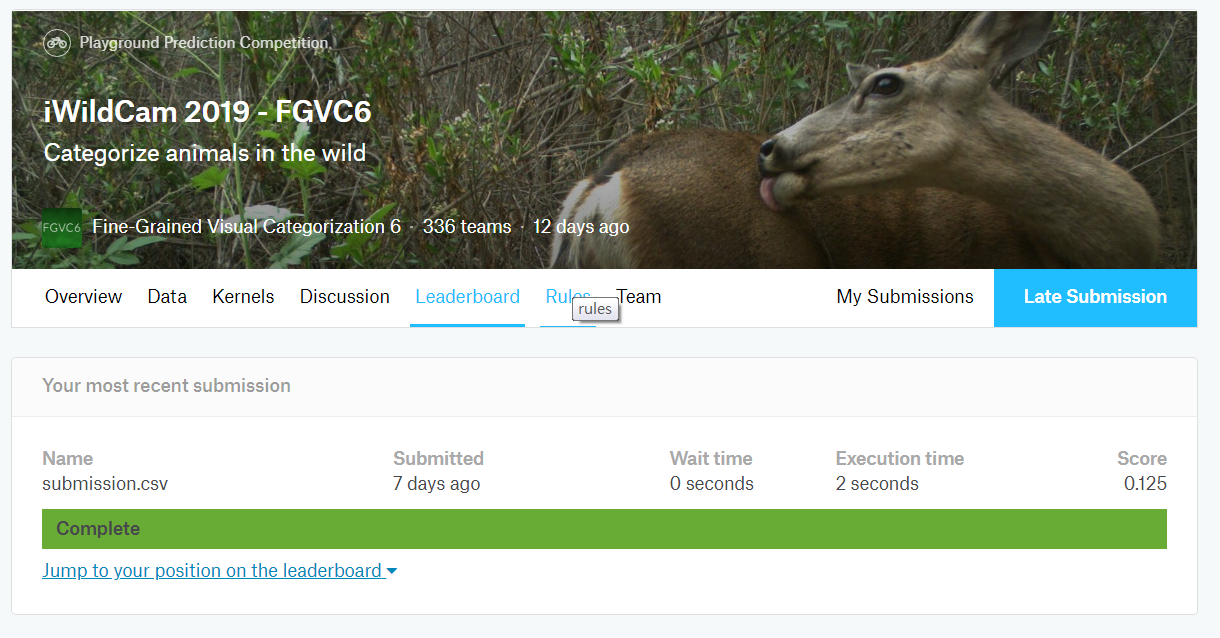
\includegraphics[width=10cm]{sorce.png}
		\end{textblock}
	}
	\end{itemize}
\end{frame}

\end{CJK}
\end{document}


